% Paste into root.tex — figures live in docs/figures/ (copy next to paper as figures/)
% On Overleaf: upload PNGs into a figures/ folder.

\begin{figure}[t]
\centering
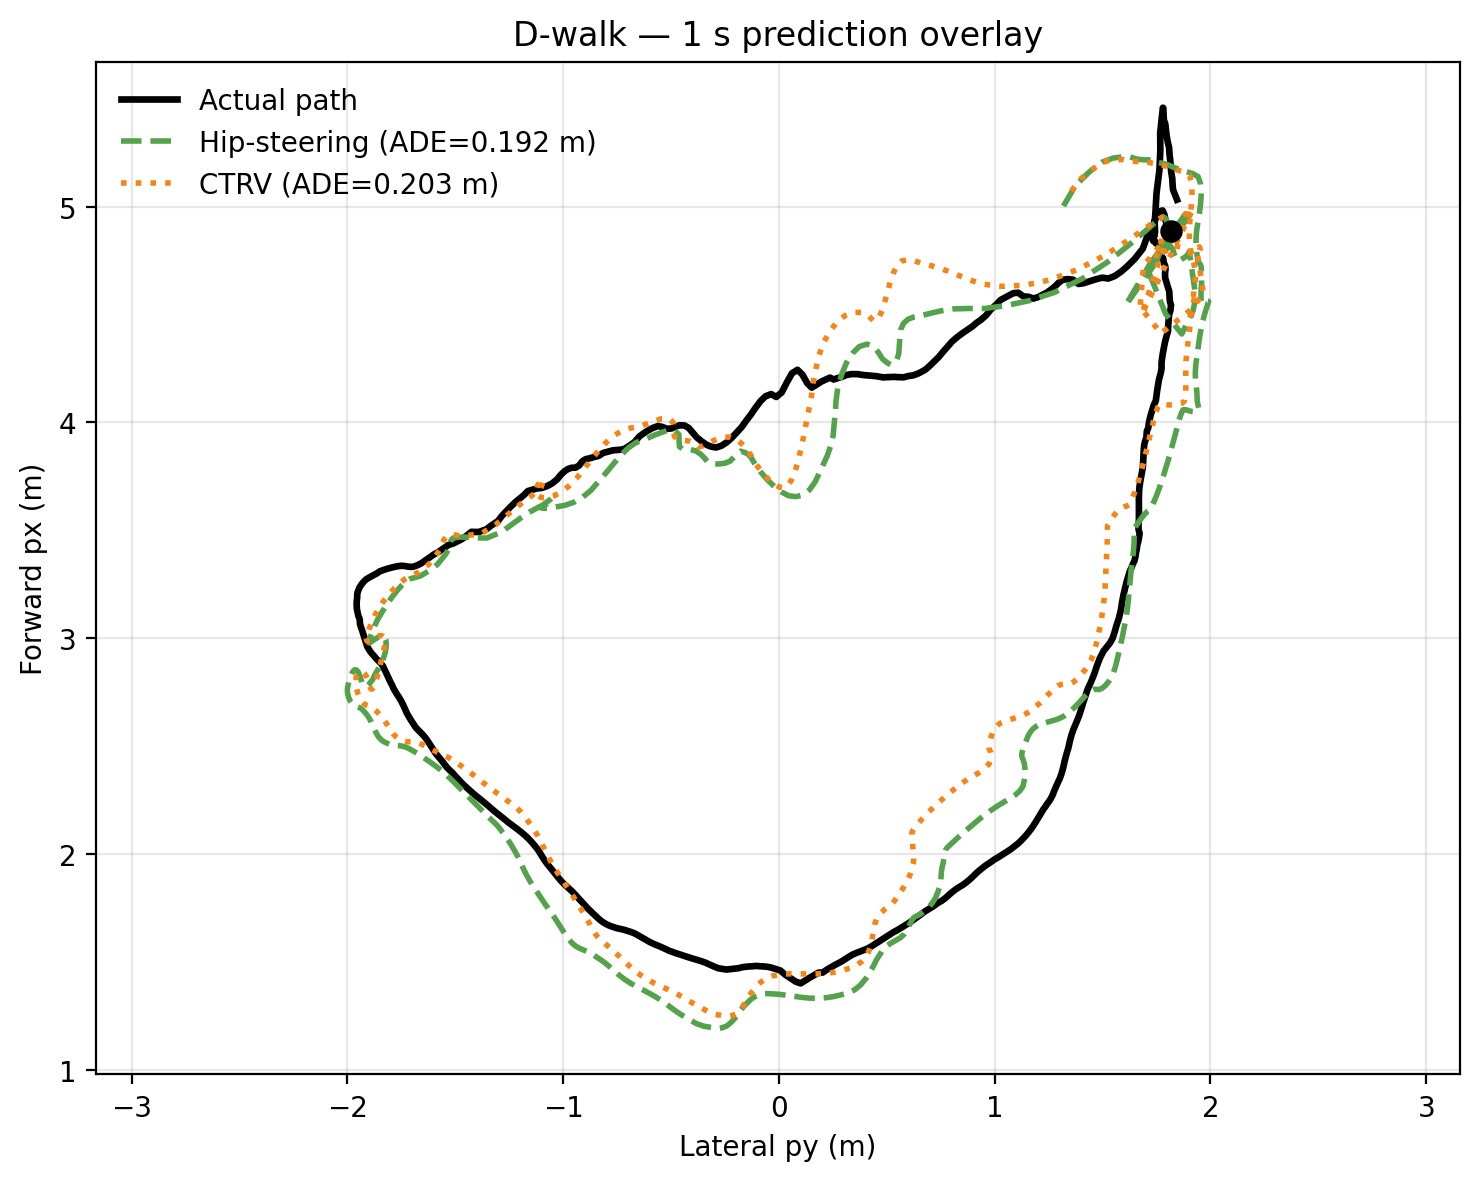
\includegraphics[width=\columnwidth]{figures/fig_dwalk_overlay.png}
\caption{D-walk $1$\,s open-loop forecast: measured path and hip-steering vs CTRV predictions.}
\label{fig:dwalk}
\end{figure}

\begin{figure}[t]
\centering
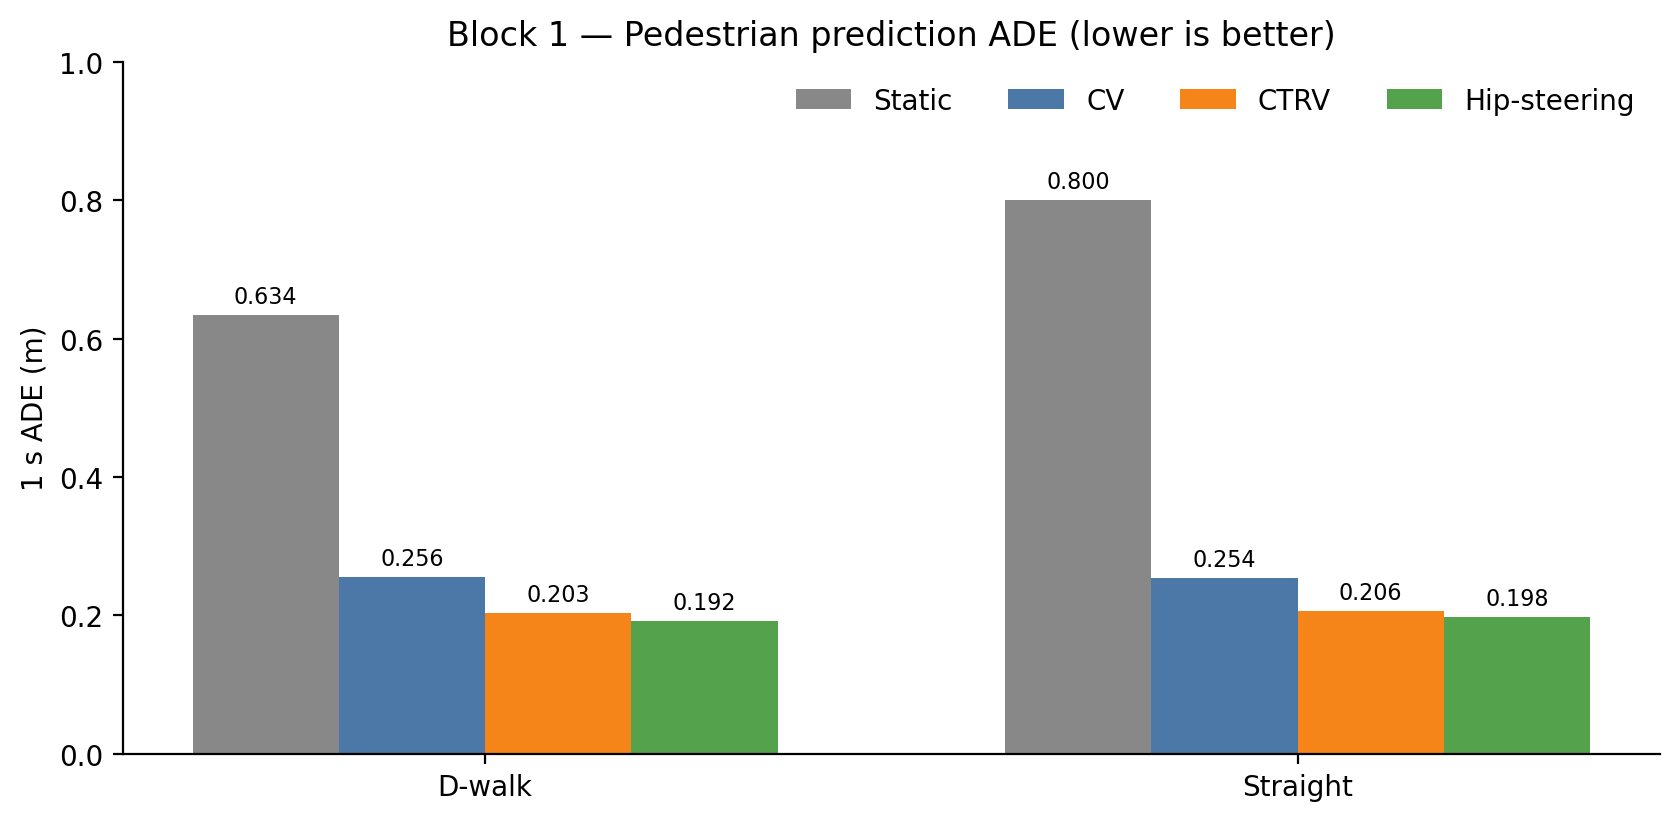
\includegraphics[width=0.95\columnwidth]{figures/fig_ade_bars.png}
\caption{Mean $1$\,s ADE on D-walk and straight SVO replays (lower is better).}
\label{fig:ade}
\end{figure}

% Optional appendix-style dashboards:
% figures/ekf_eval_dashboard_hip_Dwalk_1s.png
% figures/ekf_eval_dashboard_ctrv_Dwalk_1s.png

% Abstract tone fix (replace Nav2 sentence with):
% We also prototype publishing the forecast as a local-costmap obstacle in Nav2;
% a controlled navigation A/B study is left to future work.

% Table I stays as in root.tex (CTRV vs Hip only). To add Static/CV, see
% docs/data/block1_ade_table.txt and recompute N from the CSVs.
